\subsection{Convolutional neural network} % 2.5 pages
With the rapid development of neurobiology and cognitive science, the concept of artificial neural networks, a computational model that imitates the structure and function of biological neural networks, has been proposed as early as the last century.
\citet{fukushima1980neocognitron} proposed a network created from the animal visual system as well as some key concepts, such as \textbf{local receptive field}, \textbf{multi-layer perception architecture} and translation \textbf{equivariance and invariance property} (not affected by the shift in position).

In detail, the local receptive field means that each neuron will not perceive the image as a whole, but will only perceive the local information, then the local perception can be integrated through a multi-layer perception architecture to obtain the global perception.
On the other hand, the property of translation equivariance and invariance is emerging from the combination of the local receptive field and multi-layer perception architecture.

The study of neurobiology and cognitive science then evolved into a computational model. For example, \citet{zhang1988shift} propose the first two-dimensional Shift Invariant Artificial Neural Network (SIANN).
Then, \citet{lecun1989backpropagation} proposed a original CNN with two convolutional layers and two fully connected layers using back-propagation method to train in a supervised learning approach.
They also highlighted the term convolution for the first time, and named this model type as convolutional neural network (CNN).
Soon after the application of this model in handwritten zip code recognition, \citet{zhang1994computerized} applied it to a practical case of recognising medical imagery.

\begin{figure}[ht!]
    \centering
    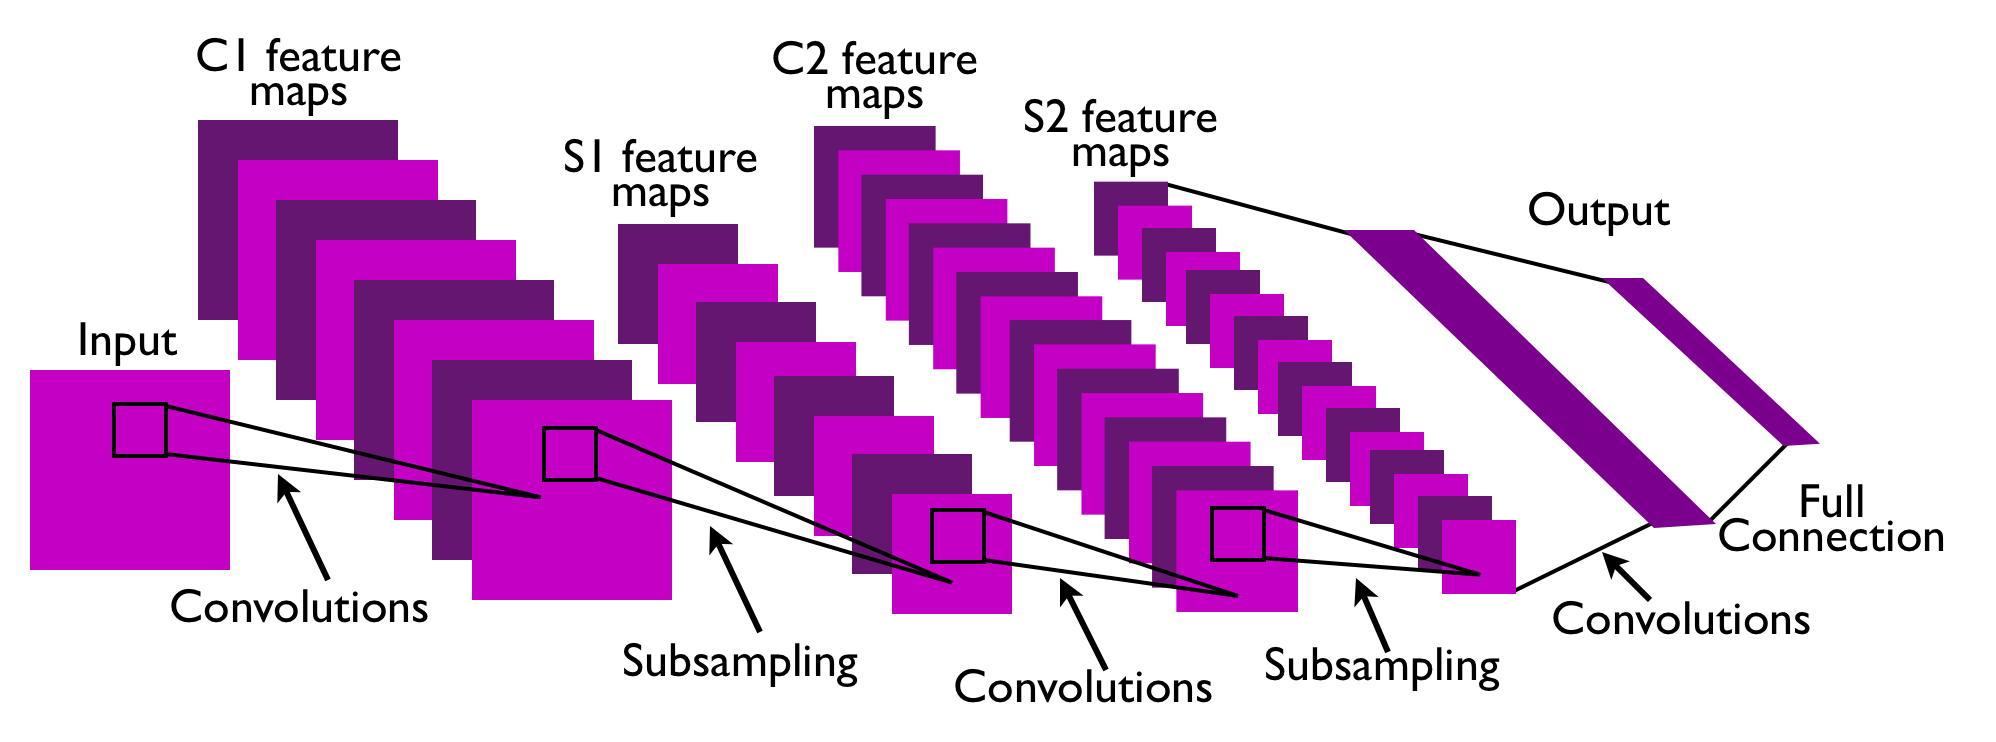
\includegraphics[width=\textwidth]{literature/imgs/ext-lecun-cnn-arch.png}
    \caption{CNN applications in vision by \citet{lecun2010convolutional}}
    \label{fig:ext-lecun-cnn-arch}
\end{figure}

The most revolutionary progress is that \citet{lecun2010convolutional} proposed a modern architecture for this model in 2010, as illustrated in figure \ref{fig:ext-lecun-cnn-arch}.
This structure comprises three convolutional layers combined in between with two sub-sampling layers, and two fully connected layers. Sub-sampling, also known as pooling, reduces the size of feature maps, by retaining only important information to simplify calculation.
Further, it further strengthens the translation invariance, taking maximum pooling as example, because the translation does not affect the maximum value, the pooling result remains unchanged.

In the following years of development of CNN, the number of layers in deep networks is gradually deepening to obtain greater high-level information.
In 2012, \citet{krizhevsky2012imagenet} proposed AlexNet which use 5 convolutional layers and 3 fully connected layers.
However, as the number of hidden layers increases, the model gets more complex and prone to overfitting.
AlexNet uses the Dropout layer by randomly breaking neuron connection (setting random input units to zero) in training process to prevent overfitting. 
Two years later, \citet{simonyan2014very} proposed Visual Geometry Group (VGG) model, in which $3\times3$ size convolution kernels are fully used in a total of 5 layers, just as the title of the paper, it is a very deep convolutional network.

The experiment in the VGG model concluded that the deeper the number of network layers, the better the performance.
However, as the depth of the model and the number of parameters continue to increase, the following two significant problems have been discovered.

\begin{enumerate}
    \item The network is prone to overfit, requiring more training data, making it more difficult to train.
    \item More storage resources and computing resources are required, but cannot provide adequate performance boost. 
\end{enumerate}

In order to solve these problems, \citet{he2015deep} proposed a residual structure to make deep network training easier with enhanced performance but fewer parameters and lower complexity. 
They first identified that the root cause of these problems is that the deeper network structure leads to degradation, i.e., the training error and the verification error both increase since the deeper network does not learn anything but loses useful features.
Then, figure \ref{fig:ext-CNN-ResNet-BBs} illustrates two types of building blocks used in ResNets with different number of layers.
The first typical block just uses cross-layer connection, a linear layer from input to output connected directly.
By denoting the desired underlying mapping as $H(x)$, the each layer learns the residual between input $x$ and desired output $F(x):=H(x)-x$.
As a result, such a residual structure allows the deep network to adapt to the appropriate depth, i.e., use the identity transform across unnecessary layers.

Further, figure \ref{fig:ext-CNN-ResNet} compares the network structure of VGG-19, 34-layer plain, and 34-layer residual and shows how to use the building block in the actual deep network. 
Figure \ref{fig:ext-CNN-ResNet-BBs} also shows a ``bottleneck'' building block for deeper ResNets, which first uses a $1\times1$ size convolution to reduce the dimensional across channels to reduce the calculation required in the $3\times3$ convolution.

\begin{minipage}[ht]{.32\textwidth}
    \begin{figure}[H]
        \centering
    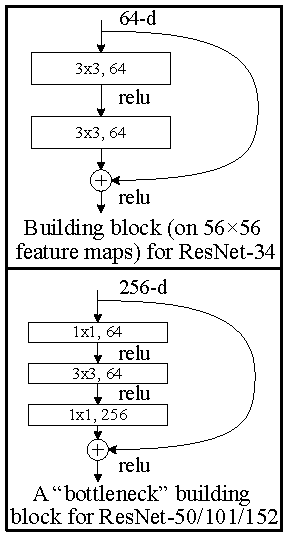
\includegraphics[width=.99\textwidth]{literature/imgs/ext-CNN-ResNet-BBs.pdf}
    \caption{Residual building blocks by \citet{he2015deep}}
    \label{fig:ext-CNN-ResNet-BBs}
    \end{figure}
\end{minipage}
\hspace{1em}
\begin{minipage}[ht]{.62\textwidth}
    \begin{figure}[H]
        \centering
    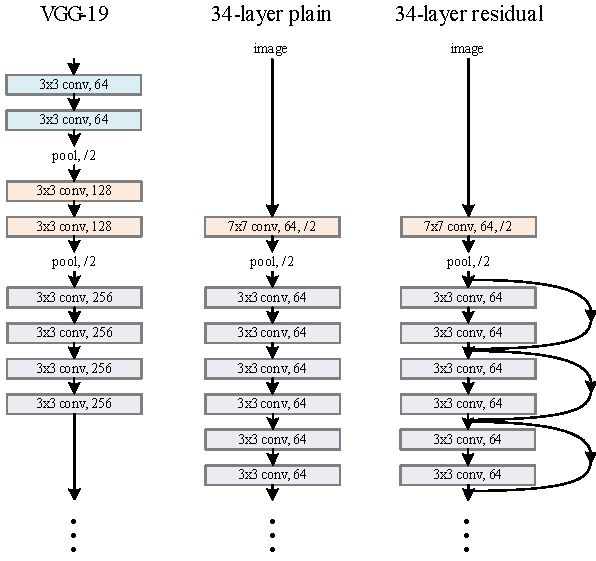
\includegraphics[width=.99\textwidth]{literature/imgs/ext-CNN-ResNet.pdf}
    \caption{VGG and Residual ImageNet by \citet{he2015deep}}
    \label{fig:ext-CNN-ResNet}
    \end{figure}
\end{minipage}